\section{Grandezze elettriche variabili nel tempo, consensatore e induttore, circuiti RC del primo ordine}

\begin{defn}[Segnale]
    Una grandezza elettrica che varia nel tempo secondo una legge determinata costituisce un segnale. 
    I segnali possono essere di tensione oppure di corrente. \\
    Un segnale è analogico quando il suo contenuto di informazione varia con
    continuità, potendo assumere un'infinità di valori possibili (entro un certo intervallo).
    Un segnale è digitale quando il suo contenuto di informazione varia in modo discreto, 
    potendo assumere soltanto un numero finito di valori possibili. \\
    Un segnale è periodico quando si ripete identicamente dopo un intervallo di tempo detto periodo.
\end{defn}

\begin{defn}[Valore medio e valore efficace]
    Il valore medio di un segnale periodico è il valore medio di una sua singola oscillazione: 
    $$V_{med} = \frac{1}{T} \int_{0}^{T} V(t) dt$$
    Il valore efficace di un segnale periodico è il valore della tensione continua che, applicata ad un resistore, 
    produce la stessa potenza dissipata dal resistore stesso quando è attraversato dal segnale periodico: 
    $$V_{eff} = \sqrt{\frac{1}{T} \int_{0}^{T} V^2(t) dt}$$
\end{defn}

\begin{defn}[Energia interna]
    Elementi circuitali il cui comportamento non dipende solo dal valore instantaneo delle grandezze elettriche, 
    ma anche dai valori assunti in precedenza, mantengono al loro interno un'informazione legata al loro funzionamento passato.
    L'informazione è fisicamente immagazzinata sotto forma di energia variabile nel tempo $w(t)$. 
    L'energia assorbita da un bipolo all'istante t è: $$w(t) = \int_{-\infty}^{t} p(\tau) d\tau$$
\end{defn}

\begin{defn}[Condensatore]
    Il condensatore è costituito da due superfici metalliche parallele separate da un isolante. 
    La carica immagazzinata è proporzionale alla tensione applicata: $$q(t) = C v(t)$$
    La costante C è la capacità del condensatore, che si misura in farad (F): $$\SI{1}{\farad} = \SI{1}{\coulomb\per\volt}$$
    Per un condensatore a facce piane e parallele di area $S$ poste ad una distanza $d$ l'una dall'altra, 
    con un dielettrico di costante dielettrica relativa $\epsilon$, la capacità è: $$C = \frac{\epsilon S}{d}$$
	\begin{figure}[H]
		\centering
		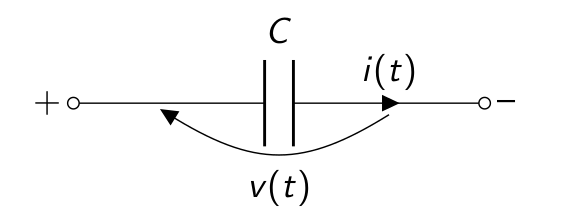
\includegraphics[width=0.5\linewidth]{figures/condensatore.png}
		\caption{Condensatore}
		\label{fig:condensatore}
	\end{figure}
    \noindent Nel condensatore la corrente è proporzionale alla derivata della tensione: $$i(t) = C \frac{dv(t)}{dt}$$
    mentre la tensione è proporzionale all'integrale della corrente: $$v(t) = \frac{1}{C} \int_{0}^{t} i(\tau) d\tau + v(0)$$
    L'energia immagazzinata nel condensatore è: $$w(t) = \frac{1}{2} C v^2(t)$$
    mentre la potenza instantanea è: $$p(t) = \frac{dw(t)}{dt} = C v(t) \frac{dv(t)}{dt}$$
\end{defn}

\begin{defn}[Induttore e legge di Faraday-Henry]
    L'induttore è costituito da un avvolgimento di filo conduttore, detto solenoide.
    All'interno dell'avvolgimento si ha un flusso magnetico $\Phi$ proporzionale alla corrente nel filo: $$\Phi(t) = L i(t)$$
    La constante $L$ è l'induttanza dell'induttore, che si misura in henry (H): $$\SI{1}{\henry} = \SI{1}{\volt\second\per\ampere}$$
	\begin{figure}[H]
		\centering
		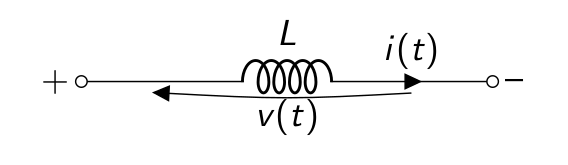
\includegraphics[width=0.5\linewidth]{figures/induttore.png}
		\caption{Induttore}
		\label{fig:induttore}
	\end{figure}
    \noindent Una variazione nel tempo del flusso magnetico produce una differenza di potenziale ai capi dell'induttore (legge di Faraday-Henry):
    $$v(t) = L \frac{di(t)}{dt}$$
    La tensione è dunque proporzionale alla derivata della corrente, mentre la corrente è proporzionale all'integrale della tensione:
    $$i(t) = \frac{1}{L} \int_{0}^{t} v(\tau) d\tau + i(0)$$
    L'energia immagazzinata nell'induttore è: $$w(t) = \frac{1}{2} L i^2(t)$$
    quindi la potenza instantanea è: $$p(t) = L i(t) \frac{di(t)}{dt}$$
\end{defn}

